\section*{Lectura 2: Demostraci\'on General del Teorema de Puntos Fijos de
Brouwer}

\begin{definition}
    Sea $X$ un subsepacio de un espacio topologico  $Y$. Decimos que  $X$ es un
     \textbf{retracto} de $Y$ s\'i existe una mapa continua $r:Y \rightarrow X$
     donde $r(x)=x$ para todo $x \in X$. Llamamos a $r$ una
     \textbf{retracci\'on} de $Y$ sobre  $X$.
\end{definition}

Es decir que el retracci\'on de $Y$ sobre $X$  lleva sus puntos fijos en todo el
$X$. Podemos ver que  $r$ es una mapa sobre, ya que $r(X)=X$ por definici\'on.

\begin{figure}[h]
    \centering
    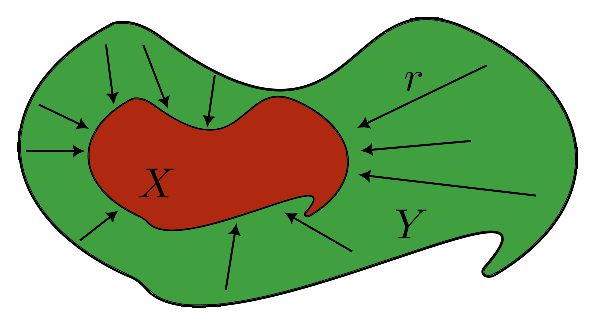
\includegraphics[scale=1.0]{Figures/retract_diagram.eps}
    \caption{Un retracci\'on $r:Y \rightarrow X$ de un espacio $Y$ hac\'ia un
    espacio  $X$.}
    \label{fig_3}
\end{figure}

Ahora recuerda que las mapas de inclusi\'on y identidad para espacios
topol\'ogicos son las mapas $i:X \rightarrow Y$ (donde $X$ es subespacio de
$Y$), y $1_X:X \rightarrow X$ dado por $i:x \rightarrow x$ y $1_X:x \rightarrow
x$ para todo $x \in X$. La definici\'on del retracto entonces se puede ver en la
siguiente diagrama, llamado una diagrama ``commutativa'':
\[\begin{tikzcd}
	&& Y \\
	\\
	\\
	X &&&& X
	\arrow["i", from=4-1, to=1-3]
	\arrow["{1_X}"', from=4-1, to=4-5]
	\arrow["r", dashed, from=1-3, to=4-5]
\end{tikzcd}\]
Entonces, seg\'un esta diagrama, $r \circ i=1_X$.

Dado una diagrama commutativa en el ``universo`` de espacios topologicos,
entonces queremos que las mapas sean mapas continuas. En este ejemplo, existe
una ``meta funci\'on`` llamado un ``functor'' $\Fc$ que lleva las espacios
topologicos hacia grupos Abelianos, tal que las diagramas commutativas son
preservada; es decir,  $\Fc$ lleva mapas continuas hacia homomorfismos.

 \begin{figure}[h]
    \centering
\[\begin{tikzcd}
	A &&&& B \\
	\\
	\\
	\\
	C
	\arrow["f", from=5-1, to=1-1]
	\arrow["g", from=1-1, to=1-5]
	\arrow["h"', from=5-1, to=1-5]
\end{tikzcd}\]
    \caption{Una diagrama commutativa, donde $A$, $B$,  $C$ son conjuntos
    cualquieras, y $f$,  $g$, y  $h$ son funciones cualquieras doned  $f \circ
g=h$.}
    \label{fig_4}
\end{figure}

\begin{lemma}\label{lemma_2.2}
    S\'i $n \geq 0$, entonces  $S^n$ no es un retracto de  $D^{n+1}$.
\end{lemma}
\begin{proof}
    Para $n=0$, es facil ver. Si  $r:D^1 \rightarrow S^0$ es un retracto,
    entonces la siguente diagrama
    \[\begin{tikzcd}
	&& {D^1} \\
	\\
	\\
	{S^0} &&&& {S^0}
	\arrow["i", from=4-1, to=1-3]
	\arrow["{1_{S^0}}"', from=4-1, to=4-5]
	\arrow["r", dashed, from=1-3, to=4-5]
\end{tikzcd}\]
nos da $r \circ i=1_{S^0}$ lo cual es imposible, ya que $S^0$ no es con\'exo, y
la imagen de  $D^1$ como subsepacio de  $S^0$ si lo es; es decir que
$r(D^1)=\{1\}$, \'o $r(D^1)=\{-1\}$. Entonces $r$ no puede ser  1--1 y sobre lo
cual contradice que  $r \circ i=1_{S^0}$ sea 1--1 y sobre.

Ahora, toma $n>0$, entonces suponga que exista una retracci\'on  $r:D^{n+1}
\rightarrow S^n$, con su diagrama de espacios topologicos y mapas continuas.
\[\begin{tikzcd}
	&& {D^{n+}} &&&&&& {H_n(D^{n+1})} \\
	\\
	\\
	{S^n} &&&& {S^n} && {H_n(S^n)} &&&& {H_n(S^n)}
	\arrow["i", from=4-1, to=1-3]
	\arrow["r", from=1-3, to=4-5]
	\arrow["{1_{S^n}}"', from=4-1, to=4-5]
	\arrow["{H_n(i)}", from=4-7, to=1-9]
	\arrow["{H_n(r)}", from=1-9, to=4-11]
	\arrow["{H_n(1_{S^n})}"', from=4-7, to=4-11]
\end{tikzcd}\]
Entonces $r \circ i=1_{s^n}$. Aplicando un functor particular llamado $H_n$,
obtemeos una diagrama commutativa de grupos Abelianos y homomorfismos. Las dos
diagramas se pueden ver arriba. Entonces tenemos que $H_n(S^n)=\Z$, y
$H_n(D^{n+1})=\vbrack{0}$. Ahora tenemos que $H_n(r) \circ
H_n(i)=H_n(1_{S^n})=1_\Z$. Esto es imposible ya que $1_\Z$ no se facotriza sobre
$\vbrack{0}$; i.e. $H_n(r) \circ H_n(i)=0 \ne 1_\Z$. Por lo tanto $S^n$ no
puede ser un retracto de  $D^{n+1}$.
\[\begin{tikzcd}
	&& \langle0\rangle \\
	\\
	\\
	\Z &&&& \Z
	\arrow["{H_n(i)}", from=4-1, to=1-3]
	\arrow["{H_n(r)}", from=1-3, to=4-5]
	\arrow["{1_\Z}"', from=4-1, to=4-5]
\end{tikzcd}\]
\end{proof}

Ahora reiteremos la teorema de Brouwer para la demostraci\'on para $n$ general.

\begin{theorem}[Teorema de Puntos Fijos de Brouwer]
    S\'i $f:D^n \rightarrow D^n$ es una funci\'on continua, entonces existe un
    punto fijo en $D^n$ para toda $n \geq 1$.
\end{theorem}
\begin{proof}
    Para $n>1$, suponga que no hay puntos fijos. Entonces sea $f:D^n \rightarrow
    D^n$ y que $f(x) \neq x$ para todo $x \in D^n$. Defina entonces, la mapa
    $g:D^n \rightarrow S^{n-1}$ dado por la figura \ref{fig_5}.
    \begin{figure}[h]
        \centering
        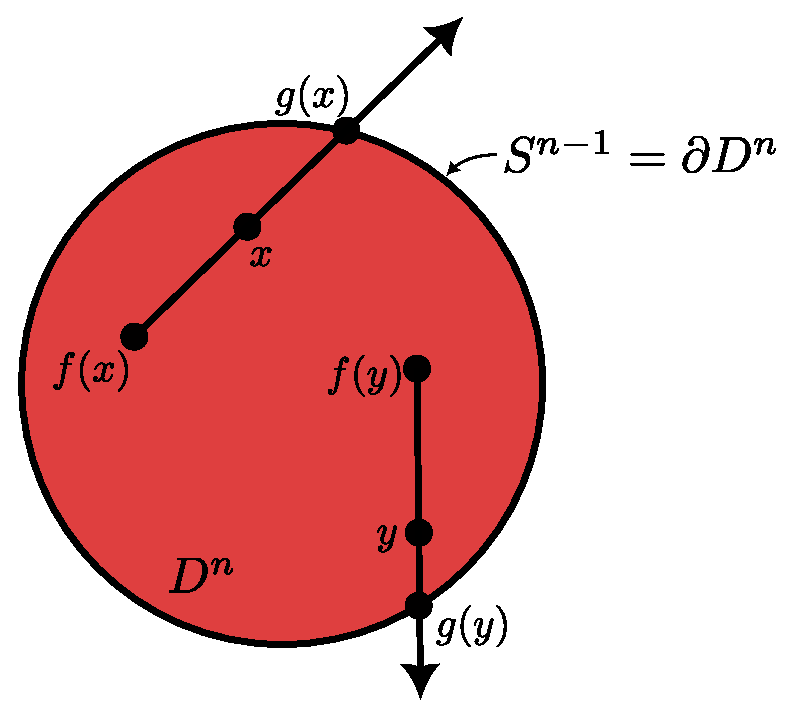
\includegraphics[scale=0.5]{Figures/brouwer_thm_2.eps}
        \caption{}
        \label{fig_5}
    \end{figure}
    Note que $g$ es continua, y que  $g(x)=x$ para todo $x \in S^{n-1}$. Puse,
    vemos que $g$ es una retracci\'on, lo cual es imposible por el lema
    \ref{lemma_2.2} Por lo tanto, no existen puntos fijos.
\end{proof}
